\documentclass[border=10pt]{standalone}
\usepackage{pgfplots}
\pgfplotsset{compat=1.18}

\begin{document}
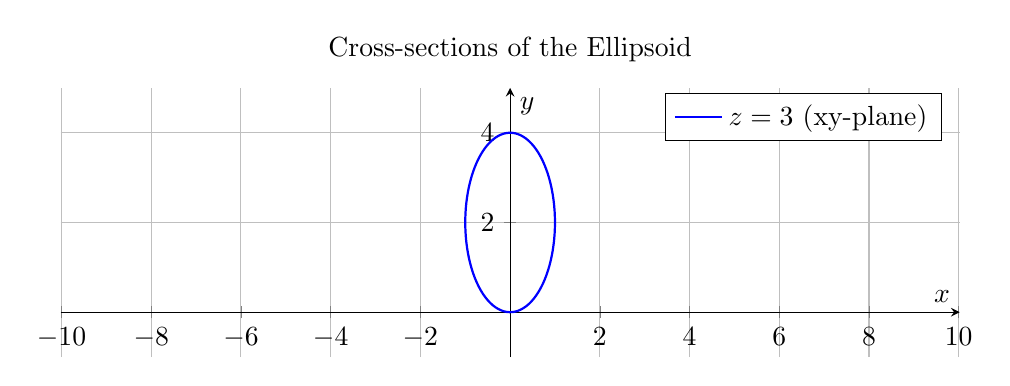
\begin{tikzpicture}
\begin{axis}[
    width=13cm,
    height=5cm,
    axis lines=center,
    grid=major,
    xlabel={$x$},
    ylabel={$y$},
    title={Cross-sections of the Ellipsoid},
    xmin=-2, xmax=2,
    ymin=-1, ymax=5,
    axis equal,
]

% Cross-section at z=3 (in xy-plane): x^2 + (y-2)^2/4 = 1
% Parametric: x = cos(t), y = 2 + 2*sin(t)
\addplot[
    domain=0:360,
    samples=100,
    blue,
    thick
] ({cos(x)}, {2 + 2*sin(x)});
\addlegendentry{$z=3$ (xy-plane)}

\end{axis}
\end{tikzpicture}

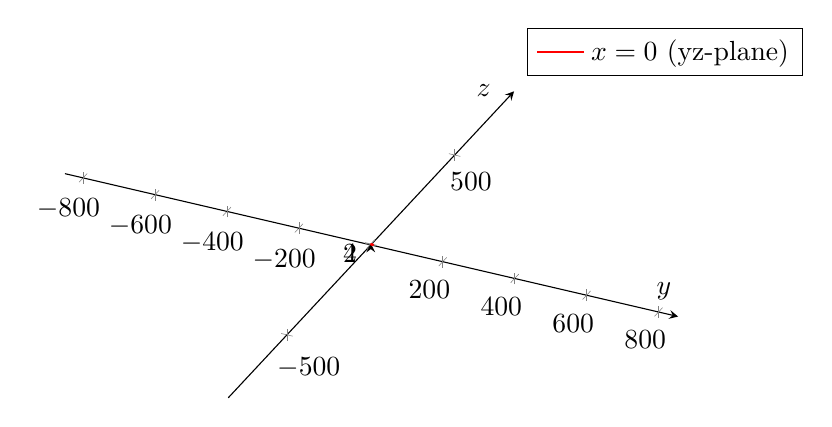
\begin{tikzpicture}
\begin{axis}[
    width=13cm,
    height=5cm,
    axis lines=center,
    grid=major,
    xlabel={$y$},
    ylabel={$z$},
    ymin=-1, ymax=5,
    zmin=1, zmax=5,
    axis equal,
]

% Cross-section at x=0 (in yz-plane): (y-2)^2/4 + (z-3)^2 = 1
% Parametric: y = 2 + 2*cos(t), z = 3 + sin(t)
\addplot[
    domain=0:360,
    samples=100,
    red,
    thick
] ({2 + 2*cos(x)}, {3 + sin(x)});
\addlegendentry{$x=0$ (yz-plane)}

\end{axis}
\end{tikzpicture}

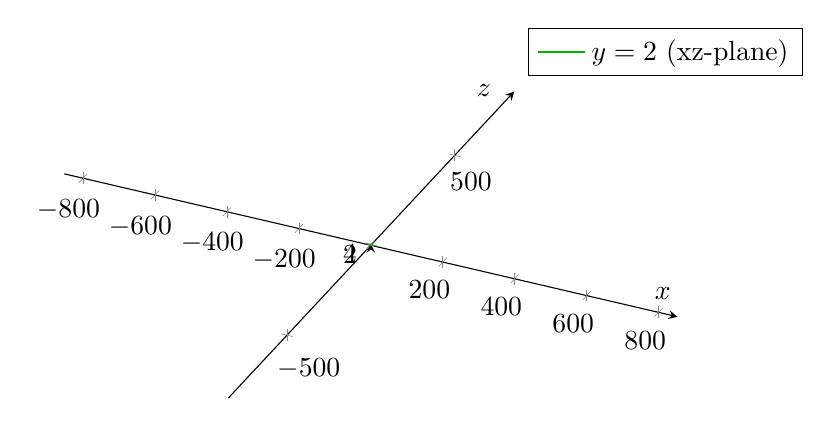
\begin{tikzpicture}
\begin{axis}[
    width=13cm,
    height=5cm,
    axis lines=center,
    grid=major,
    xlabel={$x$},
    ylabel={$z$},
    xmin=-2, xmax=2,
    zmin=1, zmax=5,
    axis equal,
]

% Cross-section at y=2 (in xz-plane): x^2 + (z-3)^2 = 1 (circle)
% Parametric: x = cos(t), z = 3 + sin(t)
\addplot[
    domain=0:360,
    samples=100,
    green!70!black,
    thick
] ({cos(x)}, {3 + sin(x)});
\addlegendentry{$y=2$ (xz-plane)}

\end{axis}
\end{tikzpicture}
\end{document}